\documentclass[hyperref, UTF8]{ctexart}

\usepackage{geometry}
\usepackage{titling}
\usepackage{titlesec}
\usepackage{paralist}
\usepackage{footnote}
\usepackage{marginnote}
\usepackage{enumerate}
\usepackage{autobreak}
\usepackage{amsmath, amssymb, amsthm}
\usepackage{mathtools}
\usepackage{bbm}
\usepackage{cite}
\usepackage{graphicx}
\usepackage{subfigure}
\usepackage{physics}
\usepackage{siunitx}
\usepackage{tikz}
\usepackage[compat=1.1.0]{tikz-feynhand}
\usepackage[ruled, vlined, linesnumbered, noend]{algorithm2e}
\usepackage[colorlinks]{hyperref} % linkcolor=black, anchorcolor=black, citecolor=black, filecolor=black
\usepackage[most]{tcolorbox}
\usepackage{caption}
\usepackage{prettyref}

\geometry{left=3.18cm,right=3.18cm,top=2.54cm,bottom=2.54cm}
\titlespacing{\paragraph}{0pt}{1pt}{10pt}[20pt]
\setlength{\droptitle}{-5em}

\DeclareMathOperator{\timeorder}{\mathcal{T}}
\DeclareMathOperator{\diag}{diag}
\DeclareMathOperator{\legpoly}{P}
\DeclareMathOperator{\primevalue}{P}
\DeclareMathOperator{\sgn}{sgn}
\newcommand*{\ii}{\mathrm{i}}
\newcommand*{\ee}{\mathrm{e}}
\newcommand*{\const}{\mathrm{const}}
\newcommand*{\suchthat}{\quad \text{s.t.} \quad}
\newcommand*{\argmin}{\arg\min}
\newcommand*{\argmax}{\arg\max}
\newcommand*{\normalorder}[1]{: #1 :}
\newcommand*{\pair}[1]{\langle #1 \rangle}
\newcommand*{\fd}[1]{\mathcal{D} #1}

\newrefformat{sec}{第\ref{#1}节}
\newrefformat{note}{注\ref{#1}}
\newrefformat{fig}{图\ref{#1}}
\newrefformat{alg}{算法\ref{#1}}
\newrefformat{back}{背景知识\ref{#1}}
\newrefformat{info}{资料框\ref{#1}}
\newrefformat{warn}{注意事项\ref{#1}}

\usetikzlibrary{arrows,shapes,positioning}
\usetikzlibrary{arrows.meta}
\usetikzlibrary{decorations.markings}
\tikzstyle arrowstyle=[scale=1]
\tikzstyle directed=[postaction={decorate,decoration={markings,
    mark=at position .5 with {\arrow[arrowstyle]{stealth}}}}]
\tikzstyle ray=[directed, thick]
\tikzstyle dot=[anchor=base,fill,circle,inner sep=1pt]

% Algorithm setting
\renewcommand{\algorithmcfname}{算法}
% Python-style code
\SetKwIF{If}{ElseIf}{Else}{if}{:}{elif:}{else:}{}
\SetKwFor{For}{for}{:}{}
\SetKwFor{While}{while}{:}{}
\SetKwInput{KwData}{输入}
\SetKwInput{KwResult}{输出}
\SetArgSty{textnormal}

\tcbuselibrary{skins, breakable, theorems}

\renewcommand{\emph}[1]{\textbf{#1}}
\newcommand*{\concept}[1]{\underline{\textbf{#1}}}


\newcommand{\Ztwo}{$\mathbb{Z}_2$}

% Cite: superscript, [1]
%\makeatletter
%\renewcommand\@citess[1]{\textsuperscript{[#1]}}
%\makeatother

\title{低维和表面物理的理论和实验}
\author{吴晋渊 18307110155}

\begin{document}

\maketitle

\section{铁磁性和低维材料}

铁磁性和反铁磁性可以粗略地分为巡游磁性和局域磁性,前者和材料中电子的费米面有关,后者涉及的电子是高度局域的,从而在能带结构中不在费米面附近。
两种机制都和电子相互作用有关\cite{annurev.ms.14.080184.000245,Cleveland_1976},直观地看,由于库仑相互作用电子气具有自旋翻转对称性,需要一定的相互作用破缺此对称性,形成铁磁或反铁磁磁性序。
此过程中允许出现的对称性破缺方式、可能出现的各种强关联效应均为值得研究的话题。

从一维Ising模型的初次提出和求解\cite{ising1925beitrag},到一维Heisenberg模型的提出和求解\cite{Bethe_1931},再到二维Ising模型\cite{onsager1944crystal},再到二维Heisenberg模型不存在铁磁相的证明\cite{PhysRevLett.17.1133},对局域磁性的理论研究经历了从经典到量子,从低维到高维,从简单的Ising模型到更加符合实际材料的Heisenberg模型的演进历程,并见证了Bethe拟设、统计场论、Mermin–Wagner定理等一系列适用范围远远超过磁性系统的理论工作的发展。

一般而言,低维体系更难发生对称性自发破缺,因为直观地看,低维下序参量的涨落的实空间关联函数$\sim \int \dd[d]{k} 1/k$具有更低的$k$幂次,从而更加容易出现红外发散,即原本可能出现的序会因为热涨落而比较容易被破坏掉。
Mermin-Wagner定理禁止在$d \leq 2$时出现任何连续对称性的破缺,因为连续对称性破缺必定出现Goldstone模,而Goldstone模的涨落在$d \leq 2$时足以破坏该连续对称性破缺导致的序——这也导致低维晶体的不稳定性,因为晶格位移的局部涨落会非常明显\cite{landau-symmetry}。%
\footnote{
    虽然$d$维量子系统等价于$d+1$维经典统计系统,但是在有限温的情况下,这个$d+1$维经典统计系统多出来的维度大小有限,从而在相变时,普适类和$d$维经典系统仍然是一样的。
    只有零温量子相变时,体系的量子性才非常重要。
}%
离散对称性不受到这个限制,二维Ising模型仍然有铁磁-顺磁相变,但一维Ising模型不存在有限温相变,在任何温度下均为顺磁性。
这个事实同样和一个更为一般的结论——van Hove定理——有关:相互作用足够局域的一维体系确实不能够发生对称性自发破缺\cite{Cuesta_2004}。
理论和数值上可以证明,自旋相互作用代数衰减的一维Ising型模型
\begin{equation}
    H = - J \sum_{\pair{i, j}} \sigma_i \sigma_j - \sum_{i, j} \frac{1}{\abs{r_i - r_j}^\alpha} \sigma_i \sigma_j
\end{equation}
由于长程相互作用,确实能够发生相变\cite{PhysRevB.54.R12661}。

因此,一个自然的问题是,一维自旋链中是否能够通过某种方式引入长程相互作用而实现铁磁序。这里的思路和前述理论工作正好相反:理论上,要严格求解一个低维模型要比严格求解一个高维模型容易,但低维系统反而在对称性自发破缺现象上有更加有趣的行为。
实际上,从提取有效模型的角度出发,三维的局域磁性主要来自交换相互作用,但低维材料中,导致局域磁性的相互作用通道还要包括偶极相互作用,并且由于衬底存在显著的各向异性,各向异性更加明显\cite{shen1997magnetism}。

文献\cite{PhysRevLett.73.898}报道说,Fe/W(110)一维链上存在铁磁序。这如果是正确的,显然是非同寻常的发现。
然而,至少两个干扰因素没有排除:实验时,在衬底上制备了多条Fe链,链和链之间可能存在偶极相互作用,而观察到的铁磁序有一定可能是非平衡现象:等待一段时间,磁性序参量会出现衰减。
\cite{shen1997magnetism}制备了一个链之间的相互作用基本可以忽略的Fe/Cu(111)链,发现其中的铁磁序确实存在时间相关的衰减,并且其变化规律可以使用以Glauber动力学更新的一维各向异性Ising模型很好地描述。
\cite{gambardella2002ferromagnetism}通过一个Co/Pt链进一步确认了这一点。因此,如果不考虑链之间的相互作用,我们获得的是所谓的“超顺磁性”,表面上的加入磁场后迅速出现磁矩的铁磁行为来自动力学因素而非平衡态因素。
实际上,\cite{PhysRevLett.73.898}报道的体系中涉及的机制比这更加有趣。对该体系进一步的研究\cite{PhysRevB.57.R677}显示,这个体系中不同的Fe链之间存在偶极相互作用,从而其低能有效模型是一个二维Ising模型,其中的每一个Ising自由度都对应单条链上由于动力学障碍形成的“短程磁畴”,从而导致一个“超铁磁序”。

总之,\cite{PhysRevLett.73.898}讨论的体系并非具有真正的铁磁序,但是它展示了远比强性加入长程相互作用更加有趣的物理机制。

\section{高温超导}

\begin{figure}
    \centering
    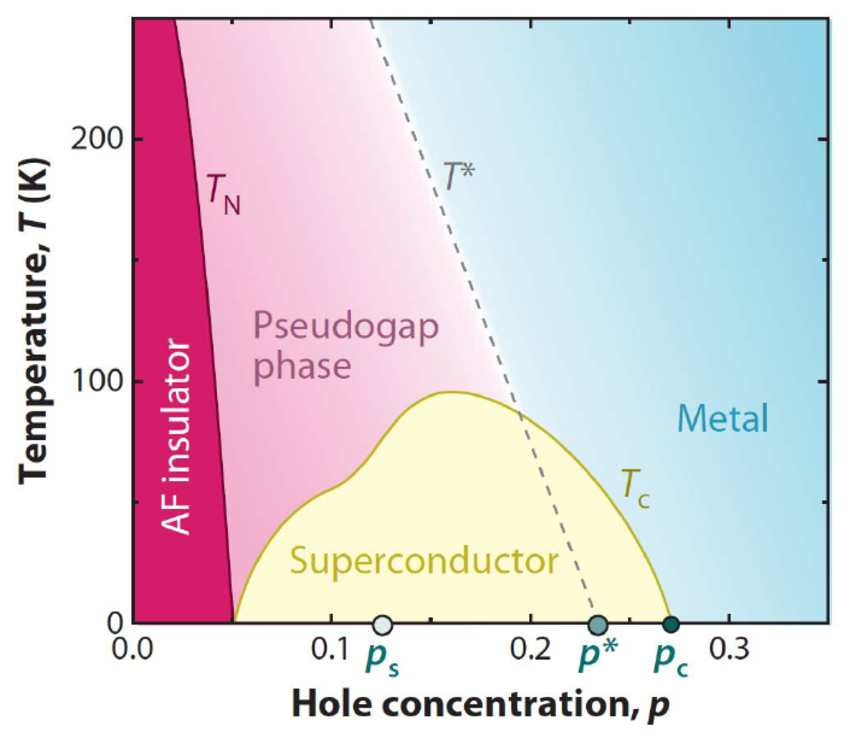
\includegraphics[width=0.6\textwidth]{phase-diagram-of-cuprate-superconductors.png}
    \caption{铜基超导体的相图示意图,取自\cite{cuprate-diagram}}
    \label{fig:cuprate}
\end{figure}

传统的BCS超导需要通过虚声子交换在电子之间形成等效吸引相互作用,来诱导电子配对,这样的等效吸引相互作用是比较弱的,从而库伯对非常容易受到热涨落破坏,超导临界温度较低。
铜氧超导能够获得高得多的超导临界温度,已经到达液氮温区,从而已有一些工程应用,如超导输电线,超导磁体(在超导线圈中产生巨大的电流,然后用它来做电磁铁)等。
然而,铜氧超导体的机制仍然是一个谜团。铜氧超导体的发现已经过去了30年,而至今理论家们还在为其机制争论不休。
除了铜基超导体以外,铁基超导体是另一类高温超导体,其行为和铜氧超导体类似但也有不同,同样没有明确的理论解释。
这些超导体的机制和之前发现的基于BCS理论的超导体显然非常不同,一方面是因为较高的临界温度,一方面是因为违反了传统超导体的Matthias规则\cite{Conder_2016}。
如\prettyref{fig:cuprate}所示,纯的铜氧材料是不导电的,是前面提到的典型的电子由于强烈的on-site排斥而高度定域,形成反铁磁态的Mott绝缘体,但在(通常是空穴)掺杂后,能够达到比常规的BCS超导体更加高的超导临界温度;如果进一步掺杂,将得到普通的金属态,超导现象消失,即如果要得到超导,并非载流子越多越好。
为何在反铁磁序的背景下引入一定的空穴就能够超导,而空穴增多反而不能超导,是一个巨大的谜团。
在超导态形成后升温超过超导临界温度,得到的并非普通的金属态,而是奇异的“赝能隙”态,其中出现了和标志着超导配对形成的超导能隙非常类似的现象,但是没有超导现象,故称为赝能隙。
赝能隙可能可以理解成电子配对已经完成,但出于某些原因没有出现超导配对的超流,于是能隙出现而没有超导,也可能可以理解成超导序在和另一种不能产生超导的电子配对序竞争。
具体发生了什么,同样是一个巨大的谜团。

Anderson的RVB理论是一种可能的通过强关联物理机制解释铜基超导的理论。所有的铜基超导体中都有CuO$_2$平面,这暗示我们,这些平面对超导的形成非常重要。
实验上,研究什么晶体结构主导了体系的电子结构是非常困难的,不过第一性原理计算的数值研究\cite{PhysRevLett.58.1028,PhysRevLett.58.1035}表明,CuO$_2$平面上的电子的确主导了铜基超导体的未掺杂母体的主要的电子行为,并且这些平面可以大致地使用一个三带Hubbard模型描述,半满时的有效理论为Heisenberg模型,即一个反铁磁Mott绝缘体,空穴掺杂时则为t-J模型,即允许一个格点上出现自旋向上、自旋向下、无电子三种情况,而双占据态由于强烈的库伦排斥不出现,空穴可以出现跳跃,从而能够载流\cite{emery1987theory}。
Anderson指出,实际上一个单带Hubbard模型就足够捕捉铜氧超导体未掺杂母体的大部分行为,如果无掺杂、半满时的Heisenberg模型存在一定阻挫,如次近邻相互作用,那么得到的基态将不是普通的具有反铁磁Neel序的Mott绝缘体,而是一个RVB态,它是一系列不同的valence band态,即格点两两配对,形成自旋单态(singlet),然后做线性叠加(即化学上所说的不同状态的“共振”)得到的状态。
将一个自旋单态解开,需要额外耗费能量。现在引入空穴,如果空穴不多,那么我们会发现,将一个自旋单态替换成两个空穴是最为节约能量的——否则需要将一个自旋单态的一个电子替换成空穴,则这个自旋单态必然被解开,会额外消耗能量。
这样,RVB态上如果引入数量合适的空穴,那么空穴会自然地形成配对,并且由于RVB态是不同的自旋单态的共振态,引入空穴后,基态也是空穴位置在不同位置的状态的共振态,即在外界扰动下,空穴可以自由移动。
如果空穴数量过少,则不能形成足够的超导配对,如果空穴数量过多,系统基态将不再由反铁磁Heisenberg模型描述,RVB态消失,从而系统行为就是普通的金属;如果空穴数量恰到好处,在低温下,空穴对发生凝聚,超导就出现了\cite{anderson1987resonating}。

Anderson的RVB理论是否就是真实情况仍然有待研究,因为其中涉及的逻辑链条非常长:CuO$_2$平面是否是最重要的物理发生的地方,单带Hubbard模型是否足够描述CuO$_2$平面,RVB态在什么参数下出现,RVB态中引入空穴而产生的空穴配对是否是主要的超导机制,这些问题每一个都有不确定之处。
为了进一步研究铜基超导体的性质,Cu$O_2$平面的直接制备和表征是非常重要的。文献\cite{zhong2016nodeless}中,作者们使用分子束外延技术在BSCCO衬底表面产生CuO$_2$薄膜,使用原位低温扫描隧道显微镜研究发现,衬底向薄膜转移不同数量的空穴时,会分别产生超导能隙和赝能隙,对赝能隙的来源做出了可能的解释,同时实验结果似乎表明铜基超导体应为$s$波超导。

\section{表面物理的实验方法}

前述工作均涉及薄膜或一维细丝材料的制备,以及对它们的表征,这些都需要表面物理的实验手段。
分子束外延(MBE)是一种常用的方法,其原理是加热容器中的超纯元素单质,产生具有很长自由程的束流,将束流导入真空室中,让不同种类的原料在晶圆衬底上发生反应并沉积出所需的薄膜\cite{cho1975molecular}。
化学气相沉积(CVD)则不使用真空室,而是将衬底依次放置在不同的前趋物中,在表面发生反应而产生薄膜\cite{pierson1999handbook}。

表面的表征手段包括扫描隧道显微镜(STM)、扫描隧道谱(STS)等。STM的原理是量子隧穿,即在势垒一端的粒子有在势垒另一端被探测到的概率,势垒越宽,概率越小,于是,通过在样品和探针之间加电场,观测流经探针的电流,就可以估测探针和样品表面的距离,移动探针,即可绘制样品表面的精细形态。
STM是非常灵敏的,甚至能够捕捉到电子云的形状,所得结果和理论预言一致\cite{stm-cloud}。
第一性原理计算可以程序化地预言STM结果,便于与实验比较\cite{vasp-stm}。
通过细致分析电流信号,还可以得到样品上各点的态密度,此即STS,它可以用于高精度地探测样品的局域性质,并分析小尺度体系如量子点的性质。

\section{结论}

虽然低维系统看起来似乎是三维的“真实”的凝聚态物理的玩具模型,但事实并非如此简单:低维系统和高维系统经常存在显著的性质不同,这些不同的实验验证本身就是重要的工作,而正如我们在一维铁磁自旋链中看到的那样,实际实验中制备的低维系统经常涉及一些出人意料的物理机制。
毫无疑问是“真实世界”的铜基超导体的研究的重头戏是对CuO$_2$平面的研究,一种较有希望的理论进路是二维Hubbard模型和自旋液体,实验研究则涉及CuO$_2$平面的制备,两者都是典型的低维物理议题。
低维系统的实验研究只能在衬底的表面上进行,这又涉及用于表征表面的各种实验技术。
低维和表面物理绝对不是琐碎或平凡的——反之,它们是凝聚态物理的核心部分之一。

\bibliographystyle{plain}
\bibliography{low-dimension-magnetization,surface-experiment,superconductivity}

\end{document}